\documentclass[letterpaper]{article}
\usepackage{aaai}
\usepackage{amsmath}
\usepackage{pgfplots}
\RequirePackage{booktabs}
\setlength{\pdfpagewidth}{8.5in} 
\setlength{\pdfpageheight}{11in}

\setcounter{secnumdepth}{0}
\pgfplotsset{compat=1.12}

\title{Automated Vacuum Cleaner Study}
\author{Rudra Sharma \and Joshua O'Dell \\ Colorado State University \\ Fort Collins, CO 80523 }
\begin{document}
\maketitle

\section{Introduction}

The purpose of this project is to simulate an automated vacuum cleaner (AUC). We will represent a room as a 2D plane which has clean and dirty points/tiles. The goal of the vacuum cleaner is to clear all the dirty points and navigate/find a path around the the room.

In the project we implement a variety of different vacuums and study its impact on performance. There have been several papers written on the study of automated vacuum cleaners. IRobot’s Roomba is an example of such a robot, we will study this implementation when developing our own algorithms.

Yap [2] explores a variety of grid based path finding algorithms, they identify an octet selection grid as an option of choosing the next point for the robot to move to as shown in figure 1. While the direct application of this paper will apply to room cleaning vacuum, these path-finding algorithms can be applied to robots searching for landmines, lawnmowers, and other agricultural tasks [3]. 

The implementation for this this project will be derived from a rudimentary implementation of a roomba robot [4]. This implementation [4] chose its next move based on a random selection from a 360$^{\circ}$ scale. We have instead opted to use the octect based selection as shown on figure 1 to choose the next tile. 

\begin{figure}[h]
	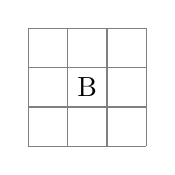
\begin{tikzpicture}
	\draw[step=.5cm,color=gray] (0,0) grid (1.5,1.5);
	\node at (+0.75,+0.75) {B};
	\end{tikzpicture}
\caption{ octet choice grid: the bot,B, has eight adjacent positions it can move to}
\label{figure:1}
\end{figure}
\section{Experiment Implementation}

The project implemented 6 distinct vacuum robots.  Each Robot has a different set of percepts, and the algorithm is adjusted to deal with it. The algorithms in each bot is a greedy algorithm with a different heuristic for calculating the cost based on the percepts the bot has. 

The following is a list of the capabilities of each Vacuum robot.
\begin{enumerate}  
\item \textbf{Preloaded Map:} Before the cleaning begins a map of the world is loaded into each the vacuum robot.
\item \textbf{Store explored nodes:} As the vacuum robot moves through the world it is allowed to store with infinite storage the tiles where it has been and the status of that tile
\item \textbf{Dirt Sensor:} A vacuum is allowed to sense the status of the tile that it is currently on.
% are we going to allow it to sense neighbors?
\item \textbf{Proximity Sensor:} the vacuum robot has the ability to know when it is close to a wall.
% assume direct neighbor, but possibly farther?
\end{enumerate}  


\subsection{Random Bot}

\begin{tabular}{ r | l }  
	Preloaded map 		& No \\
	Store explored 		& No \\
	Proximity 		 	& No \\
	sensor 					 \\
\end{tabular}
\quad
\begin{tabular}{ r | l }  
	Observable		& Unobservable 	\\
	Deterministic	& Deterministic \\
	Episodic		& Sequential	\\
	Static		 	& Static 		\\
	Discrete 		& Discrete 		\\
	Agents		 	& Single 		\\
\end{tabular}
The Random robot was the first Robot we implemented for our study. This robot has no form of storage or sensors to guide it in cleaning a room. 
When the robot is initialized, it will clean the location it is placed on and then it will randomly select a next point based on what is adjacent to it, thereby giving it eight options. See fig. 1 for display of the Octet grid selection for the random robot. 



\subsection{Store Map Bot}

\begin{tabular}{ r | l }  
	Preloaded Map 		& Yes \\
	Store explored 		& No \\
	Proximity  		 	& No \\
	sensor 					 \\
\end{tabular}
\quad
\begin{tabular}{ r | l }  
	Observable 		& Fully 		\\
	Deterministic 	& Deterministic \\
	Episodic		& Sequential	\\
	Static		 	& Static 		\\
	Discrete 		& Discrete 		\\
	Agents		 	& Single 		\\	
\end{tabular}
The preloaded map was a Robot which was given the the exact boundaries of the room prior to start. The objective of this robot was to use its knowledge of the boundaries of the room to avoid attempting to go outside the boundaries of the room. This robot was an extension to the random robot so the path that it choose next was also a random selection from the octet grid, however it knows to avoid the points in the objects which represent points outside the boundaries of the room.

\subsection{Store Map with Direction Bot}
\begin{tabular}{ r | l }  
	Preloaded Map 		& Yes \\
	Store explored		& No \\
	Proximity 		 	& No \\
	sensor 					 \\
\end{tabular}
\quad
\begin{tabular}{ r | l }  
	Observable		& Fully 		\\
	Deterministic	& Deterministic \\
	Episodic		& Sequential	\\
	Static		 	& Static 		\\
	Discrete 		& Discrete 		\\
	Agents		 	& Single 		\\	
\end{tabular}
The store map with direction was an extension to the store map. However, this map no longer had a random element which decided its next point in the room. Instead it uses a strategy of maintaining a direction until it reaches the boundary of a room. After it reaches a boundary it will side to the adjacent slide and do a 180 degree turn and travel in the the opposite direction it came from until it hits the opposite boundary of the room. It will keep repeating this process until it completes the entire room.

\subsection{Proximity Bot}

\begin{tabular}{ r | l }  
	Preloaded Map 		& No \\
	Store Explored 		& No \\
	Dirt Sensor 		& Yes \\
	Proximity  		 	& Yes \\
	sensor 					 \\
\end{tabular}
\quad
\begin{tabular}{ r | l }  
	Observable		& Partially		\\
	Deterministic	& Deterministic \\
	Episodic		& Sequential 	\\
	Static		 	& Static 		\\
	Discrete 		& Discrete 		\\
	Agents		 	& Single 		\\	
\end{tabular} 
 	
 		
 		
This program was implemented by mimicking the `Roomba''s algorithm.  The algorithm creates a spiral from the starting position outward.  Once the proximity sensor detects a wall the algorithm changes.  The new algorithm will choose a random direction, and continue straight along that direction until the proximity sensor detects another wall, at which point another random direction is chosen.  

The largest hurdle with this program was finding the best equation to calculate a spiral.  At each step in the simulation a new direction was calculated using the following equation.
$ 22.5 - (\mathrm {e} ^ x * 45)$
where time x was decremented by $0.01$ during each step.  The program in theory appeared to be quite efficient, however when run we saw that it had difficulty even completing a 10\% in a timely manner.  I attribute this to some tweaking that is necessary on the spiral formula.  I believe it is going over the same places too much, however given our grid approach any more aggressive spiraling would result in a missed grid item in the center.


\subsection{Stored Explored Bot}

\begin{tabular}{ r | l }  
	Preloaded Map 		& No \\
	Store explored 		& Yes \\
	Dirt Sensor 		& No \\
	Proximity 		 	& No \\
	sensor 					 \\
\end{tabular}
\quad
\begin{tabular}{ r | l }  
	Observable 		& Unobservable 	\\
	Deterministic 	& Deterministic \\
	Episodic		& Sequential	\\
	Static		 	& Static 		\\
	Discrete 		& Discrete 		\\
	Agents		 	& Single 		\\	
\end{tabular}
This program is allowed to maintain a list of the grid spaces where it has visited.  It is allowed to know where each of these grid places are in relation to its current location.
The algorithm used in this program will attempt to try and keep the vacuum close to the grid items that were previously visited.  To do this the following steps are taken.  
\begin{enumerate}  
\item Get a list of all the possible steps we can take.
\item for each step determine a ranking.  This is calculated by summing the distance to each of the existing items.
\item choose the step with the highest rank.
\end{enumerate}

If a spot is chosen that is outside of the grid, the program essentially loses a turn.  We also try to avoid revisiting gird places where we have already been.  To do this if a possible location turns up in our visited list, then we increase the rank.  Essentially moving the rank high enough that other options even if they move away from the existing cluster will be chosen.  Thus the rank equation is as follows.

\[
  Rank=
	\begin{cases}
		visited=False: \sum{distance(visited)}\\
		visited=True: sizeOf(Visited)
	\end{cases}
\]

\subsection{Store Explored + Proximity Bot}

\begin{tabular}{ r | l }  
	Preloaded Map 		& No \\
	Store explored 		& Yes \\
	Dirt Sensor 		& No \\
	Proximity 		 	& Yes \\
	sensor 					 \\
\end{tabular}
\quad
\begin{tabular}{ r | l }  
	Observable		& Partially 	\\
	Deterministic	& Deterministic	\\
	Episodic		& Sequential	\\
	Static		 	& Static 		\\
	Discrete 		& Discrete 		\\
	Agents		 	& Single 		\\	
\end{tabular}
This program is an extension of the `store explored' program.  One of the things we noticed about the store explored was that depending on where it started we could get into a situation where we had finished the middle of the room, and 1 side, but needed to complete the other side.  To do this we have to cross the already cleaned region, which our algorithm did not handle elegantly.

Adding a proximity sensor the the vacuum robot allowed us to do the following.  When the robot first starts cleaning it chooses a single direction.  Once it reaches a wall it then begins the existing algorithm from the `store explored' robot.  This the robot can start cleaning on 1 side of the room, and not have to back track.  The result was improved cleaning times.

\section{Results}
\begin{table}[h!]
\begin{tabular}{ r | l l l l l }  
					& 10\%		& 50\%		& 80\%		& 100\%		\\
	\midrule
	Random			& 96\% 		& 77\% 		& 40\%		& 12\%		\\
	Store Map		& 100\%		& 100\% 	& 100\%  	& 100\% 	\\
	Store Map 		& 100\%		& 100\% 	& 100\%  	& 100\% 	\\
	with direction \\
	Proximity		& 40\%		& 34\% 		& 27\%  	& 25\% 		\\
	Store Explored 	& 100\%		& 100\% 	& 100\%  	& 100\% 	\\
	Store Explored 	& 100\%		& 100\% 	& 100\%  	& 100\% 	\\
	with proximity 	\\
\end{tabular}
\caption{Percent success (depth = 1,000,000)}
\label{table:1}
\end{table}

\begin{table}[h!]
\begin{tabular}{ r | l l l l l }  
					& 10\%		& 50\%		& 80\%		& 100\%		\\
	\midrule
	Random			& 146783 	& 680976 	& 894746 	& 1000000	\\
	Store Map		& 373		& 3895 		& 9006  	& 42284 	\\
	Store Map 		& 160		& 947 		& 1756 		& 2408		\\
	with direction \\
	Proximity		& 600159	& 732261 	& 759790 	& 906491	\\
	Store Explored 	& 535		& 8491		& 22586		& 39161		\\
	Store Explored 	& 539		& 3857 		& 7163 		& 16898		\\	
	with proximity 	\\
\end{tabular}
\caption{Actual steps taken to complete (depth = 1,000,000)}
\end{table}

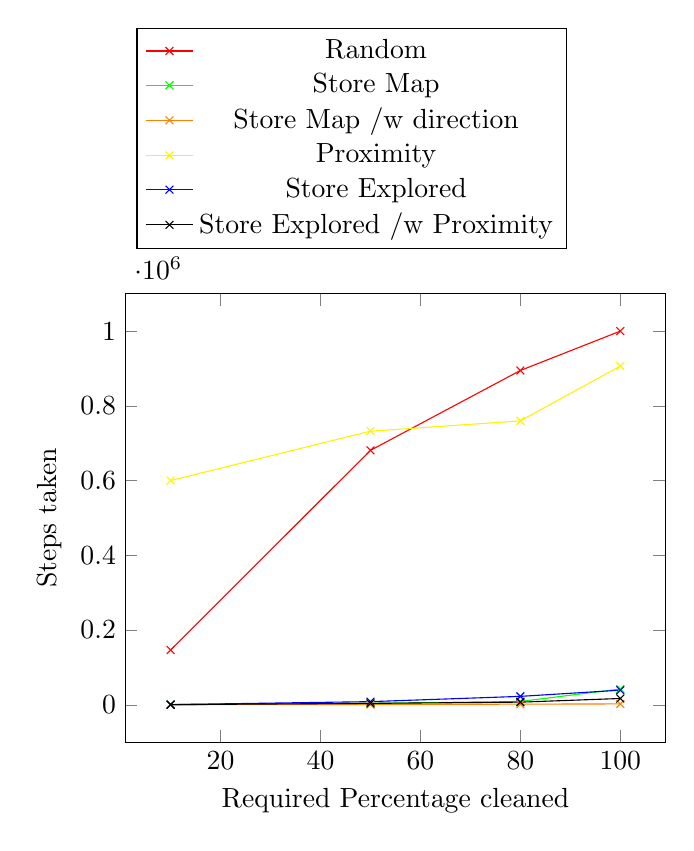
\begin{tikzpicture}
	\begin{axis}[
		xlabel=Required Percentage cleaned,
		ylabel=Steps taken,
		legend style={at={(0.02,1.1)},anchor=south west}]
	\addplot[color=red,mark=x] coordinates {
 		(  10,   146783)
 		(  50,   680976)
 		(  80,   894746)
 		( 100,  1000000)
	};
	\addlegendentry{Random}
	\addplot[color=green,mark=x] coordinates {
 		(  10,   373)
 		(  50,  3895)
 		(  80,  9006)
 		( 100, 42284)
	};
	\addlegendentry{Store Map}
	\addplot[color=orange,mark=x] coordinates {
 		(  10,   160)
 		(  50,   947)
 		(  80,  1756)
 		( 100,  2408)
	};
	\addlegendentry{Store Map /w direction}
	\addplot[color=yellow,mark=x] coordinates {
 		(  10,  600159)
 		(  50,  732261)
 		(  80,  759790)
 		( 100,  906491)
	};
	\addlegendentry{Proximity}
	\addplot[color=blue,mark=x] coordinates {
 		(  10,    535)
 		(  50,   8491)
 		(  80,  22586)
 		( 100,  39161)
	};
	\addlegendentry{Store Explored}
	\addplot[color=black,mark=x] coordinates {
 		(  10,    539)
 		(  50,   3857)
 		(  80,   7163)
 		( 100,  16898)
	};
	\addlegendentry{Store Explored /w Proximity}
	\end{axis}
\end{tikzpicture}





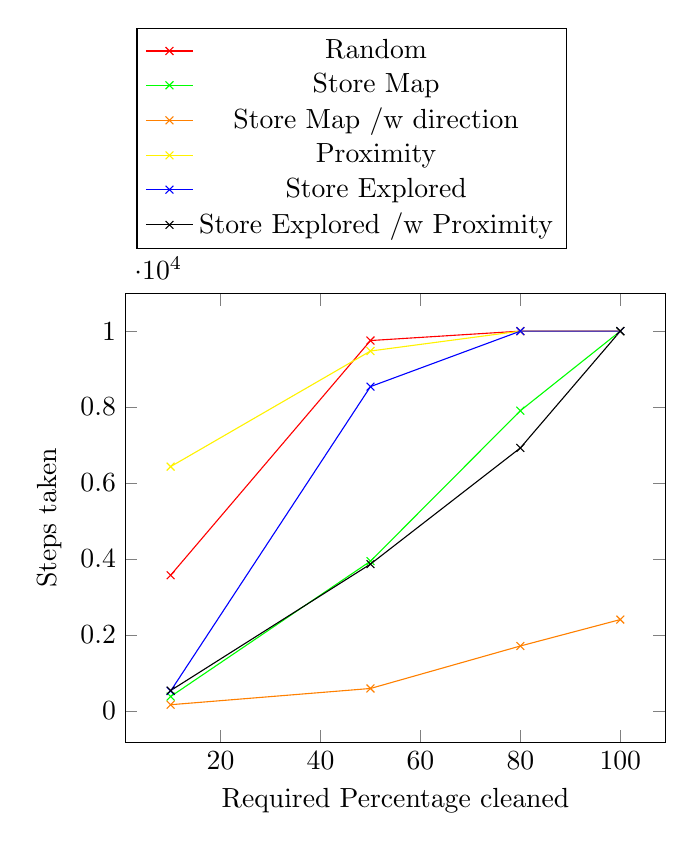
\begin{tikzpicture}
	\begin{axis}[
		xlabel=Required Percentage cleaned,
		ylabel=Steps taken,
		legend style={at={(0.02,1.1)},anchor=south west}]
	\addplot[color=red,mark=x] coordinates {
 		(  10,   3570)
 		(  50,   9752)
 		(  80,  10000)
 		( 100,  10000)
	};
	\addlegendentry{Random}
	\addplot[color=green,mark=x] coordinates {
 		(  10,   375)
 		(  50,  3941)
 		(  80,  7905)
 		( 100, 10000)
	};
	\addlegendentry{Store Map}
	\addplot[color=orange,mark=x] coordinates {
 		(  10,   160)
 		(  50,   588)
 		(  80,  1707)
 		( 100,  2403)
	};
	\addlegendentry{Store Map /w direction}
	\addplot[color=yellow,mark=x] coordinates {
 		(  10,   6431)
 		(  50,   9476)
 		(  80,  10000)
 		( 100,  10000)
	};
	\addlegendentry{Proximity}
	\addplot[color=blue,mark=x] coordinates {
 		(  10,    520)
 		(  50,   8539)
 		(  80,  10000)
 		( 100,  10000)
	};
	\addlegendentry{Store Explored}
	\addplot[color=black,mark=x] coordinates {
 		(  10,    533)
 		(  50,   3864)
 		(  80,   6924)
 		( 100,  10000)
	};
	\addlegendentry{Store Explored /w Proximity}
	\end{axis}

\end{tikzpicture}





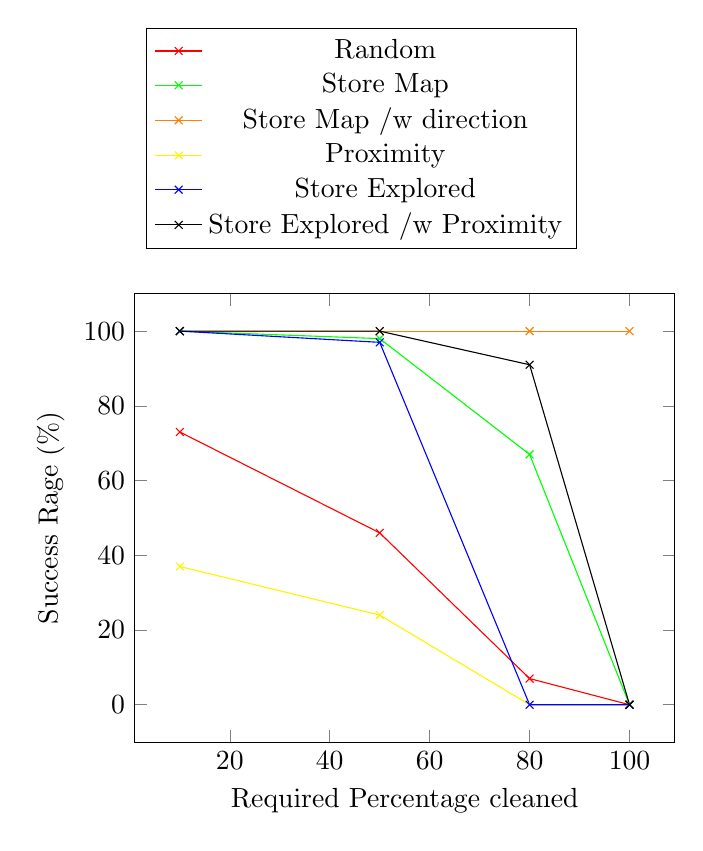
\begin{tikzpicture}
	\begin{axis}[
		xlabel=Required Percentage cleaned,
		ylabel=Success Rage (\%),
		legend style={at={(0.02,1.1)},anchor=south west}]
	\addplot[color=red,mark=x] coordinates {
 		(  10, 73)
 		(  50, 46)
 		(  80,  7)
 		( 100,  0)
	};
	\addlegendentry{Random}
	\addplot[color=green,mark=x] coordinates {
 		(  10, 100)
 		(  50,  98)
 		(  80,  67)
 		( 100,   0)
	};
	\addlegendentry{Store Map}
	\addplot[color=orange,mark=x] coordinates {
 		(  10,  100)
 		(  50,  100)
 		(  80,  100)
 		( 100,  100)
	};
	\addlegendentry{Store Map /w direction}
	\addplot[color=yellow,mark=x] coordinates {
 		(  10, 37)
 		(  50, 24)
 		(  80,  0)
 		( 100,  0)
	};
	\addlegendentry{Proximity}
	\addplot[color=blue,mark=x] coordinates {
 		(  10, 100)
 		(  50,  97)
 		(  80,   0)
 		( 100,   0)
	};
	\addlegendentry{Store Explored}
	\addplot[color=black,mark=x] coordinates {
 		(  10,  100)
 		(  50,  100)
 		(  80,   91)
 		( 100,   0)
	};
	\addlegendentry{Store Explored /w Proximity}
	\end{axis}

\end{tikzpicture}



\begin{tabular}{ r | l }  
	\toprule
		& avg \% cleaned \\
	\midrule
	P1	& 15 \\
	P2	& 45 \\
	P3	& 84 \\
	P4	& 56 \\
	P5	& 77 \\
	P6	& 1 \\
	\bottomrule
\end{tabular}

\section{Conclusion}
\ref{table:1}
% \cite[p. 2] {Optimized_Path_Planning}
\listoftables
\listoffigures
\nocite{*}
\bibliography{report}
\bibliographystyle{aaai}
\end{document}


